\section{Data Analysers}\label{section:analysers}

A data analyser is a component that consumes posts and produces per-post analysis. Socneto comes with two major analysis components: Topic modelling and Sentiment analysis. The implementation is common for both components. The functionality that is different is discussed in  Chapter \ref{chapter:analysis}.

\subsection{Requirements and Dependencies}

Data acquirers require the following tools for its proper function:

\begin{itemize}
    \item Kafka 2.4.0
    \item python 3.8
    \item Topic modelling trained model: en\_core\_web\_lg-2.2.5\footnote{\url{https://github.com/explosion/spacy-models/releases/download/en_core_web_lg-2.2.5/en_core_web_lg-2.2.5.tar.gz}} downloaded automatically upon building
    \item Trained sentiment model, also downloaded upon building.
\end{itemize}

They communicate with the following services:
\begin{itemize}
    \item Storage service (see Section \ref{section:storage})
    \item Job management service (see Section \ref{section:jms})
\end{itemize}

\subsection{Code}

The code wrapping libraries discussed in Chapter \ref{chapter:analysis} can be found in the \texttt{main.py} file. There are three notable functions:

\begin{itemize}
    \item \texttt{register\_itself} - sends registration requests (see Section \ref{subsection:registrationrequest}) whose attributes contains element \texttt{outputFormat} with the structure of format of the output analysis.
    \item \texttt{process\_acquired\_data} -  starts consuming topic where posts appear.
    \item \texttt{analyse} - invokes analysis.
\end{itemize}

\subsection{Build + Run}

\textbf{Topic modelling}:
\begin{itemize}
    \item \texttt{pip install -r requirements.txt} - installs requirements
    \item \texttt{wget -O en\_core\_web\_lg-2.2.5.tar.gz https://github.com/explosion/spacy-models/releases/download/en\_core\_web\_lg-2.2.5/en\_core\_web\_lg-2.2.5.tar.gz} - downloads the topic modelling trained model.
    \item \texttt{pip install en\_core\_web\_lg-2.2.5.tar.gz} - installs the model
    \item \texttt{python main.py}
\end{itemize}
 
\subsection{Configuration}

The script \texttt{main.py} accepts the following parameters:

\begin{itemize}
    \item \texttt{--server\_address} - address of the Kafka server
    \item \texttt{--input\_topic} - topic from which the analysers consume the posts.
    \item \texttt{--output\_topic} - topic to which the analysers produce analysis for the post (not the post itself). Set to the database input topic.
    \item \texttt{--registration\_topic} - topic to which the registration request is sent.
\end{itemize}

\subsection{Communication}\label{subsection:ds_communication}
\begin{figure}[H]
    \centering
    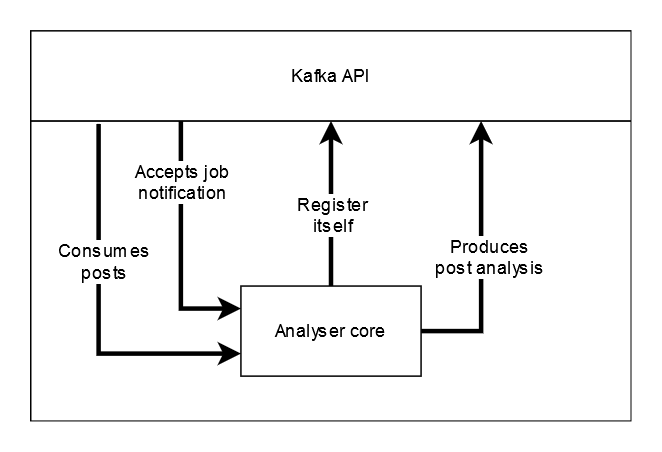
\includegraphics[width=0.8\textwidth]{diagrams/api-ds.png}
    \caption{Kafka interface is used to listen to job notification, produce analysis and register the component}
    \label{fig:apiDs}
\end{figure}
JMS uses Kafka for the communication depicted in Figure \ref{fig:apiDs}



\subsubsection{Kafka Interface}\label{subsubsection:ds_kafkainterface}

The simplicity of the analysers allows them to ignore job notifications. The only entity they consume is a post (see Appendix \ref{subsection:postmessage}) which has been already discussed in detail in Section \ref{section:da_outgoing}.

\subsubsection{Outgoing Communication}

\paragraph{Registration}\label{subsubsection:registration_analyser}

An analyser needs to register itself on startup. The registration request was already discussed in Section \ref{subsubsection:jms_kafkainterface}. The only addition is that they in element \texttt{outputFormat}.

\paragraph{Output format} Every analyser can produce any number of results, but the result value has to have one of the six possible formats:
\begin{itemize}
    \item \texttt{textValue} - a single string value
    \item \texttt{numberValue} - a single number value
    \item \texttt{textListValue} - a list of string values
    \item \texttt{numberListValue} - a list of number values
    \item \texttt{textMapValue} - a map of a string key and a string value
    \item \texttt{numberMapValue} - a map of a string key and a string value  
\end{itemize}
During registration each analyser has to pass a map with result name and its value type. This information is used during a chart definition on FE. The result has to be always in this format (see \ref{analysis} Analysis paragraph).

\paragraph{Analysis}\label{analysis}

Analysers produce analysis entity (see Appendix \ref{section:analysisMessage}) with the following fields:

\begin{itemize}
    \item \texttt{postId} - Guid of the related post
    \item \texttt{jobId} - Id of the job in which context this post was produced
    \item \texttt{componentId} - Analysers component Id
    \item \texttt{results} - Actual result of the analysis enclosed in an element with the analysis name.
\end{itemize}

\vspace{3\baselineskip}
Example - sentiment analysis: 

\begin{lstlisting}[language=json,firstnumber=1]
{
  "postId": "1234dsfgdsf",
  "jobId": "4df8165f-9461-4cdc-b6bc-b5fa0414319b",
  "componentId": "s_analyser_1",
  "results": {
    "polarity": {
        "numberValue": 1,
        "textValue": null,
        "numberListValue": null,
        "textListValue": null,
        "numberMapValue": null,
        "textMapValue": null
    }
  }
}
\end{lstlisting}
\newpage
Example - topic modelling: 

\begin{lstlisting}[language=json,firstnumber=1]
{
  "postId": "1234dsfgdsf",
  "jobId": "4df8165f-9461-4cdc-b6bc-b5fa0414319b",
  "componentId": "topic_analyser_1",
  "results": {
    "polarity": {
        "numberValue": null,
        "textValue": null,
        "numberListValue": null,
        "textListValue": ['food','bread',...],
        "numberMapValue": null,
        "textMapValue": null
    }
  }
}
\end{lstlisting}

